\chapter{Симметрия и законы сохранения}

\lectureoverview{Стационарное действие и уравнения Эйлера--Лагранжа составляют одну половину сердца классической механики; гамильтонова формулировка — другую. Здесь мы разовьём первую половину настолько, чтобы выявить глубокую закономерность: каждая непрерывная симметрия лагранжиана порождает сохраняющуюся величину. Мы обнаружим эту закономерность на примере трансляций и вращений, докажем её для общего бесконечно малого преобразования, а затем внимательно рассмотрим, где этот аргумент применим, а где нет.}

\section{Минимум математики, объясняющий физику}

Записи, уже имеющиеся на доске, могут немного напоминать уравнение Шрёдингера, но это не тема сегодняшнего вечера. Тема — симметрия и законы сохранения. Нет честного способа объяснить их связь без уравнений. Сами уравнения элементарны; важно расположить их так, чтобы структура стала видимой. В Scientific American результат можно просто назвать, но здесь нам нужен минимум математики, необходимый, чтобы вывести его так, как это делают физики.

Введём малый параметр \(\epsilon\). Мы сохраняем члены, пропорциональные \(\epsilon\), и отбрасываем \(O(\epsilon^2)\). Это сокращённая запись предельного перехода, а не утверждение, будто у ненулевого действительного числа буквально нулевой квадрат. Для обычной функции \(f(x,y)\),
\begin{equation}
  \delta f
  =\frac{\partial f}{\partial x}\,\delta x
   +\frac{\partial f}{\partial y}\,\delta y
   +O(\epsilon^2),
  \label{eq:first-variation-f}
\end{equation}
где и \(\delta x\), и \(\delta y\) пропорциональны \(\epsilon\). Обозначение \(\delta f\) означает изменение \(f\), а не произведение числа, называемого \(\delta\), на \(f\). Для стационарной точки выполняется
\begin{equation}
  \delta f=0
  \qquad\hbox{to first order.}
  \label{eq:stationary-f}
\end{equation}

Для механической траектории \(q_i(t)\) аналогичной величиной является действие
\begin{equation}
  S[q]=\int_{t_1}^{t_2}L(q,\dot q,t)\,dt.
  \label{eq:action-l4}
\end{equation}
Варьирование траектории при фиксированных концах даёт
\begin{equation}
  \delta S
  =\int_{t_1}^{t_2}dt\,
   \sum_i\left(
     \frac{\partial L}{\partial q_i}\,\delta q_i
     +\frac{\partial L}{\partial\dot q_i}\,\delta\dot q_i
   \right).
  \label{eq:action-variation-l4}
\end{equation}
Эти два члена возникают потому, что изменение траектории изменяет и координаты, и скорости. Интегрирование по частям вместе с условием
\(\delta q_i(t_1)=\delta q_i(t_2)=0\) превращает \(\delta S=0\) в
\begin{equation}
  \frac{d}{dt}\left(\frac{\partial L}{\partial\dot q_i}\right)
  -\frac{\partial L}{\partial q_i}=0.
  \label{eq:el-l4}
\end{equation}

\begin{figure}[htbp]
  \centering
  \includegraphics[width=0.76\textwidth]{lecture_04_figure_05.png}
  \caption{Уравнение Эйлера--Лагранжа, напомненное как отправная точка для симметрии и законов сохранения.}
  \lectureframe{00:09:00}
\end{figure}

Правильное выражение — \emph{стационарное действие}, а не обязательно наименьшее действие. К этому различию мы вернёмся ближе к концу.

\section{Обобщённые координаты и сопряжённый импульс}

Декартовы координаты положения — слишком узкий язык для общей механики. Координатами могут быть положения частиц, углы, коллективные переменные или амплитуды полей, поэтому мы обозначаем их как \(q_i\). Лагранжиан — это сжатое задание динамики. Даже Стандартная модель, если записать её без очень сжатых обозначений, занимает примерно страницу; запись отдельного уравнения движения для каждой компоненты поля заняла бы несравненно больше. Одна функция \(L\) объединяет всё это.

Сопряжённый к \(q_i\) импульс равен
\begin{equation}
  p_i=\frac{\partial L}{\partial\dot q_i}.
  \label{eq:canonical-momentum-l4}
\end{equation}
Вот почему обобщённые координаты традиционно называют \(q\): соответствующие импульсы — это \(p\), так что у нас получаются наши \(p\) и \(q\). В этих обозначениях уравнение~\eqref{eq:el-l4} принимает вид
\begin{equation}
  \dot p_i=\frac{\partial L}{\partial q_i}.
  \label{eq:momentum-el-l4}
\end{equation}

Для привычной одномерной частицы,
\begin{equation}
  L=\frac{m\dot x^2}{2}-V(x),
  \qquad
  \frac{\partial L}{\partial\dot x}=m\dot x,
  \label{eq:particle-momentum-l4}
\end{equation}
так что сопряжённый импульс совпадает с обычным импульсом.

\begin{figure}[htbp]
  \centering
  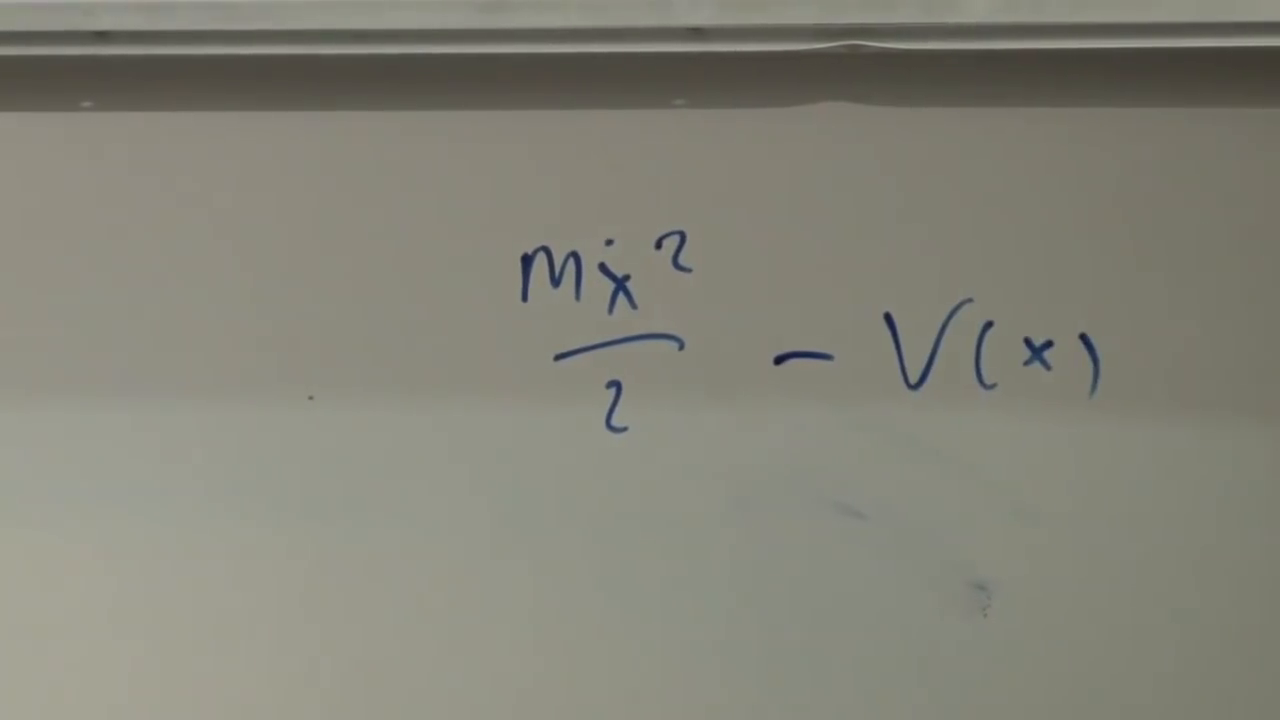
\includegraphics[width=0.72\textwidth]{lecture_04_figure_02.png}
  \caption{Лагранжиан вида «кинетическая энергия минус потенциальная», используемый для отождествления сопряжённого импульса с \(m\dot x\).}
  \lectureframe{00:14:48}
\end{figure}

Если \(q_i\) не входит в \(L\), то \(\dot p_i=0\). Это привычный путь от циклической координаты к закону сохранения. Однако настоящая связь более общая, и полезно сначала обнаружить её на примерах, прежде чем доказывать.

\section{Законы сохранения, обнаруженные до их объяснения}

\subsection{Две координаты и потенциал, зависящий от разности координат}

Положим обе массы равными единице и возьмём
\begin{equation}
  L=\frac{\dot q_1^{\,2}+\dot q_2^{\,2}}{2}-V(q_1-q_2).
  \label{eq:separation-lagrangian}
\end{equation}
Можно представить себе две частицы на прямой. Их взаимодействие зависит только от разности их координат.

\begin{figure}[htbp]
  \centering
  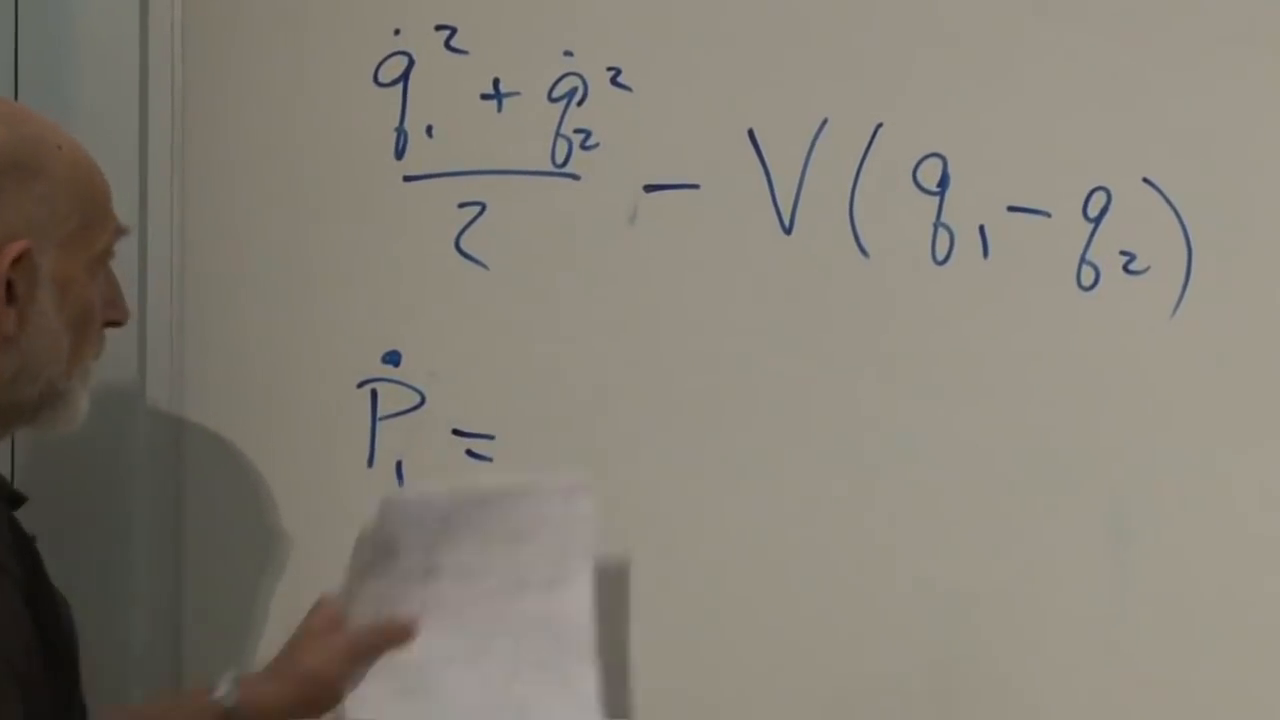
\includegraphics[width=0.78\textwidth]{lecture_04_figure_03.png}
  \caption{Лагранжиан с двумя координатами и начало первого уравнения для импульса.}
  \lectureframe{00:18:56}
\end{figure}

Обозначая через \(V'\) производную по аргументу \(V\),
\begin{align}
  \dot p_1&=-V'(q_1-q_2),
  \notag\\
  \dot p_2&=+V'(q_1-q_2).
  \label{eq:separation-momentum-equations}
\end{align}
Знак во втором уравнении меняется на противоположный, потому что увеличение \(q_2\) уменьшает \(q_1-q_2\).

\begin{classroomqa}
  \audiencequestion{Должно ли первое уравнение для импульса содержать \(V'\), и откуда берётся его знак минус?
  \lecturetimestamp{00:20:52--00:21:35}}
  \lecturerresponse{Уравнение Эйлера--Лагранжа утверждает \(\dot p_1=\partial L/\partial q_1\), а не то, что лагранжиан равен нулю. Поскольку \(L=T-V\), дифференцирование по \(q_1\) даёт \(-V'\). Дифференцирование по \(q_2\) даёт ещё один знак минус из \(q_1-q_2\), поэтому во втором уравнении стоит \(+V'\).}
\end{classroomqa}

\begin{figure}[htbp]
  \centering
  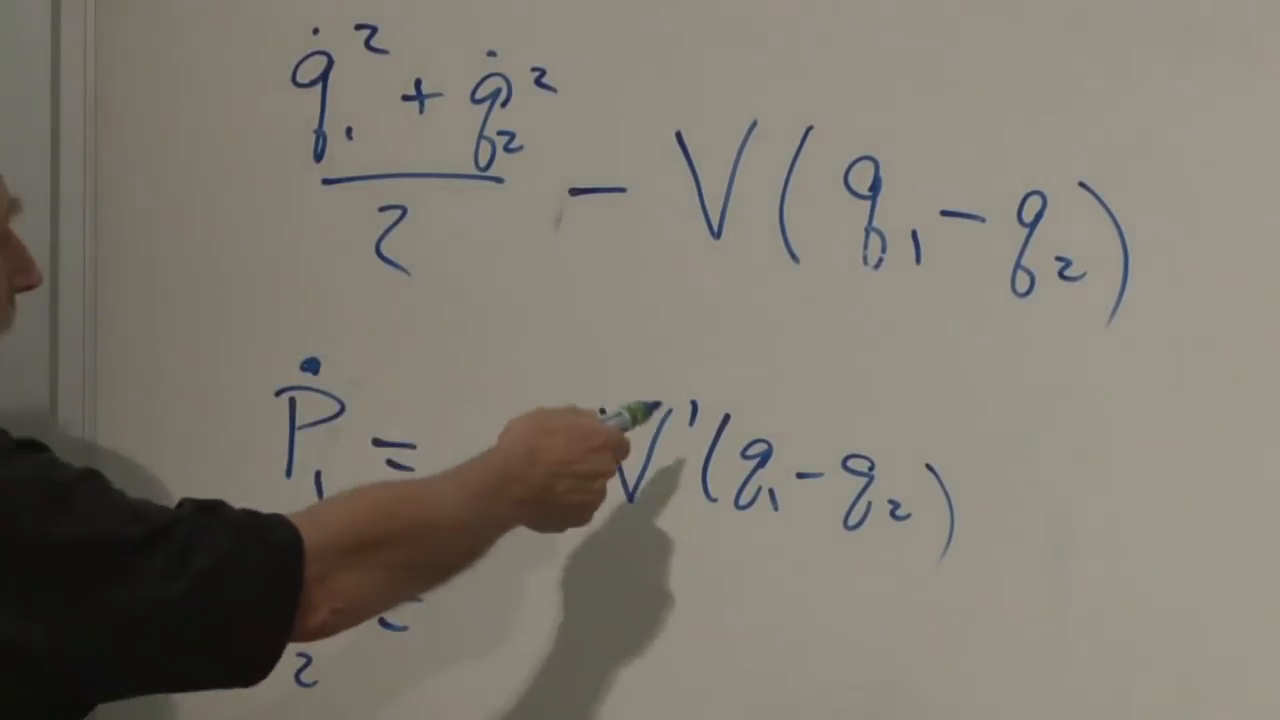
\includegraphics[width=0.78\textwidth]{lecture_04_figure_04.png}
  \caption{Чувствительная к знаку производная в уравнении для \(p_1\); уравнение для \(p_2\) получает противоположный знак.}
  \lectureframe{00:20:41}
\end{figure}

Складывая уравнения~\eqref{eq:separation-momentum-equations}, получаем
\begin{equation}
  \frac{d}{dt}(p_1+p_2)=0.
  \label{eq:total-p-conserved}
\end{equation}
Мы нашли сохраняющуюся величину, но ещё не объяснили, почему она существует.

\subsection{Менее очевидная линейная комбинация}

Теперь пусть
\begin{equation}
  L=\frac{\dot q_1^{\,2}+\dot q_2^{\,2}}{2}
    -V(Aq_1+Bq_2),
  \label{eq:ab-lagrangian}
\end{equation}
где \(A\) и \(B\) — константы. Тогда
\begin{align}
  \dot p_1&=-A\,V'(Aq_1+Bq_2),
  \notag\\
  \dot p_2&=-B\,V'(Aq_1+Bq_2).
  \label{eq:ab-momentum-equations}
\end{align}
Умножая первое уравнение на \(B\), второе на \(A\) и вычитая, исключаем силу:
\begin{equation}
  \frac{d}{dt}(Bp_1-Ap_2)=0.
  \label{eq:ab-conserved}
\end{equation}

\begin{figure}[htbp]
  \centering
  \includegraphics[width=0.78\textwidth]{lecture_04_figure_06.png}
  \caption{Взвешенные уравнения для импульса, в которых силовые члены сокращаются в \(Bp_1-Ap_2\).}
  \lectureframe{00:24:20}
\end{figure}

\begin{classroomqa}
  \audiencequestion{Откуда физически могут возникнуть такие константы, как \(A\) и \(B\)?\lecturetimestamp{00:25:09--00:30:15}}
  \lecturerresponse{Рассмотрим две частицы масс \(m\) и \(M\):
  \[
    L=\frac{m\dot X^2}{2}+\frac{M\dot Y^2}{2}-V(X-Y).
  \]
  Перейдём к \(Q_1=\sqrt m\,X\) и \(Q_2=\sqrt M\,Y\). Кинетический член становится \((\dot Q_1^2+\dot Q_2^2)/2\), тогда как потенциал зависит от \(Q_1/\sqrt m-Q_2/\sqrt M\). Таким образом, неодинаковые массы естественно становятся коэффициентами линейной комбинации. Замена \(Q_2\) на \(-Q_2\) меняет показанный минус на плюс, не изменяя квадратичного кинетического члена.}
\end{classroomqa}

\begin{figure}[htbp]
  \centering
  \includegraphics[width=0.82\textwidth]{lecture_04_figure_07.png}
  \caption{Координаты, взвешенные массами, упрощают кинетическую энергию, перенося массовые множители в потенциал.}
  \lectureframe{00:28:40}
\end{figure}

\begin{classroomqa}
  \audiencequestion{Показывает ли это, что сохраняющаяся величина может существовать без циклической координаты?\lecturetimestamp{00:31:13--00:31:58}}
  \lecturerresponse{В записанных переменных нет \emph{очевидной} циклической координаты. Замена переменных может её выявить, но искать её здесь — не самый полезный подход. Аргумент, основанный на симметрии, прямо укажет сохраняющуюся комбинацию.}
\end{classroomqa}

\section{Что мы понимаем под симметрией}

\subsection{Трансляции}

Начнём со свободной частицы единичной массы,
\begin{equation}
  L=\frac{\dot q^2}{2}.
  \label{eq:free-unit-l4}
\end{equation}
Сдвинем каждую точку её траектории на одну и ту же константу:
\begin{equation}
  q'(t)=q(t)+\epsilon.
  \label{eq:free-translation}
\end{equation}
Поскольку \(\epsilon\) не зависит от времени, \(\dot q'=\dot q\), и потому \(\delta L=0\). Эта инвариантность и есть трансляционная симметрия.

Есть две эквивалентные картины. В пассивной мы сдвигаем начало координат, оставляя объект фиксированным. В активной мы оставляем оси фиксированными и перемещаем объект. Активный язык окажется менее запутывающим: переместим физическую конфигурацию и спросим, замечает ли это \(L\).

Для формулы~\eqref{eq:separation-lagrangian} сдвинем обе координаты:
\begin{equation}
  \delta q_1=\epsilon,
  \qquad
  \delta q_2=\epsilon.
  \label{eq:common-translation}
\end{equation}
Скорости не меняются, и \(q_1-q_2\) тоже.

\begin{figure}[htbp]
  \centering
  \includegraphics[width=0.78\textwidth]{lecture_04_figure_08.png}
  \caption{Общая трансляция оставляет разность двух координат неизменной.}
  \lectureframe{00:35:30}
\end{figure}

Для формулы~\eqref{eq:ab-lagrangian} используем менее очевидное преобразование
\begin{equation}
  \delta q_1=B\epsilon,
  \qquad
  \delta q_2=-A\epsilon.
  \label{eq:ab-transformation}
\end{equation}
Снова скорости не меняются, а
\begin{equation}
  \delta(Aq_1+Bq_2)=AB\epsilon-BA\epsilon=0.
  \label{eq:ab-invariant-argument}
\end{equation}
Следовательно, это преобразование является симметрией.

\begin{figure}[htbp]
  \centering
  \includegraphics[width=0.80\textwidth]{lecture_04_figure_09.png}
  \caption{Асимметричная трансляция, сохраняющая \(Aq_1+Bq_2\).}
  \lectureframe{00:40:20}
\end{figure}

\begin{classroomqa}
  \audiencequestion{Коэффициенты кодируют массы, так что сохраняющаяся величина становится обычным импульсом центра масс?
  \lecturetimestamp{00:42:25--00:42:45}}
  \lecturerresponse{Да. В переменных, взвешенных по массам, симметрия и сохраняющаяся комбинация выглядят несимметрично. При обратном переходе к \(X\) и \(Y\) восстанавливаются обычный одновременный перенос и полный импульс.}
\end{classroomqa}

\subsection{Повороты}

Рассмотрим одну частицу на плоскости,
\begin{equation}
  L=\frac{m}{2}(\dot x^2+\dot y^2)-V(x^2+y^2).
  \label{eq:central-lagrangian-l4}
\end{equation}
Это центральный потенциал. Мы сравниваем две фиксированные системы координат, повернутые друг относительно друга; оси не вращаются со временем. При одном согласованном выборе ориентации,
\begin{align}
  x'&=x\cos\theta+y\sin\theta,
  \notag\\
  y'&=-x\sin\theta+y\cos\theta.
  \label{eq:finite-rotation-l4}
\end{align}

\begin{figure}[htbp]
  \centering
  \includegraphics[width=0.82\textwidth]{lecture_04_figure_10.png}
  \caption{Лагранжиан для центрального потенциала и две фиксированные декартовы системы координат, связанные поворотом.}
  \lectureframe{00:45:40}
\end{figure}

Положим \(\theta=\epsilon\) и сохраним члены первого порядка:
\begin{equation}
  \cos\epsilon=1+O(\epsilon^2),
  \qquad
  \sin\epsilon=\epsilon+O(\epsilon^3).
  \label{eq:small-angle-l4}
\end{equation}
Тогда бесконечно малый поворот имеет вид
\begin{align}
  \delta x&=y\epsilon,
  &\delta y&=-x\epsilon,
  \notag\\
  \delta\dot x&=\dot y\epsilon,
  &\delta\dot y&=-\dot x\epsilon.
  \label{eq:infinitesimal-rotation-l4}
\end{align}

\begin{figure}[htbp]
  \centering
  \includegraphics[width=0.82\textwidth]{lecture_04_figure_11.png}
  \caption{Бесконечно малый поворот координат и скоростей.}
  \lectureframe{00:49:50}
\end{figure}

В отличие от переноса, величина изменения \(x\) зависит от \(y\), а величина изменения \(y\) зависит от \(x\). Тем не менее,
\begin{align}
  \delta(x^2+y^2)
  &=2x\,\delta x+2y\,\delta y=0,
  \notag\\
  \delta(\dot x^2+\dot y^2)
  &=2\dot x\,\delta\dot x+2\dot y\,\delta\dot y=0.
  \label{eq:rotation-invariants-l4}
\end{align}
И потенциальный, и кинетический члены инвариантны.

\begin{figure}[htbp]
  \centering
  \includegraphics[width=0.76\textwidth]{lecture_04_figure_12.png}
  \caption{Сокращение в первом порядке, показывающее, что квадрат радиуса инвариантен относительно поворотов.}
  \lectureframe{00:53:20}
\end{figure}

\section{Общая теорема о сохранении}

Примеры с переносом и поворотом имеют одну общую форму. Пусть непрерывное бесконечно малое преобразование имеет вид
\begin{equation}
  \delta q_i=\epsilon f_i(q),
  \qquad
  \delta\dot q_i=\frac{d}{dt}\delta q_i,
  \label{eq:general-infinitesimal-symmetry}
\end{equation}
где \(\epsilon\) не зависит от времени, а \(f_i\) может зависеть от всех координат.

\begin{figure}[htbp]
  \centering
  \includegraphics[width=0.78\textwidth]{lecture_04_figure_13.png}
  \caption{Общее поле бесконечно малых смещений
  \(\delta q_i=\epsilon f_i(q)\).}
  \lectureframe{00:56:00}
\end{figure}

Вариация лагранжиана в первом порядке равна
\begin{equation}
  \delta L
  =\sum_i\left(
    \frac{\partial L}{\partial q_i}\delta q_i
    +\frac{\partial L}{\partial\dot q_i}\delta\dot q_i
  \right).
  \label{eq:delta-l-general}
\end{equation}

\begin{figure}[htbp]
  \centering
  \includegraphics[width=0.84\textwidth]{lecture_04_figure_14.png}
  \caption{Два вклада в \(\delta L\): вариация координат и вариация скоростей.}
  \lectureframe{01:02:30}
\end{figure}

Теперь ограничимся физической траекторией, так что выполняются уравнения Эйлера--Лагранжа. Используя
\begin{equation}
  \frac{\partial L}{\partial\dot q_i}=p_i,
  \qquad
  \frac{\partial L}{\partial q_i}=\dot p_i,
  \label{eq:el-substitution-l4}
\end{equation}
получаем
\begin{align}
  \delta L
  &=\sum_i\left(\dot p_i\,\delta q_i
                +p_i\,\delta\dot q_i\right)
  \notag\\
  &=\frac{d}{dt}\sum_i p_i\delta q_i
  =\epsilon\frac{d}{dt}\sum_i p_i f_i(q).
  \label{eq:noether-derivation-l4}
\end{align}
Ключевой шаг здесь — всего лишь правило произведения.

Если преобразование является симметрией, то \(\delta L=0\). Поскольку \(\epsilon\) — произвольный постоянный множитель,
\begin{equation}
  \boxed{
  \frac{d\mathcal Q}{dt}=0,
  \qquad
  \mathcal Q=\sum_i p_i f_i(q)}
  .
  \label{eq:noether-charge-l4}
\end{equation}
Это — ядро теоремы Нётер в классической механике для точных, не зависящих от времени точечных симметрий.

\begin{figure}[htbp]
  \centering
  \includegraphics[width=0.84\textwidth]{lecture_04_figure_15.png}
  \caption{Шаг с правилом произведения, который превращает инвариантность \(L\) в сохраняющуюся величину.}
  \lectureframe{01:05:00}
\end{figure}

\begin{classroomqa}
  \audiencequestion{В \(f_i(q)\) должен ли \(q\) иметь ещё один индекс?
  \lecturetimestamp{01:06:57--01:07:31}}
  \lecturerresponse{Обозначение \(q\) без индекса означает весь набор
  \((q_1,q_2,\ldots)\). Каждая компонента \(f_i\) может зависеть от всех этих
  координат. Например, для поворота \(f_x=y\) и \(f_y=-x\).}
\end{classroomqa}

Теперь эти примеры перестают быть случайными. Для одновременного переноса
\(f_1=f_2=1\), поэтому
\begin{equation}
  \mathcal Q=p_1+p_2.
  \label{eq:noether-common-p}
\end{equation}
Для несимметричного переноса \(f_1=B\), \(f_2=-A\), поэтому
\begin{equation}
  \mathcal Q=Bp_1-Ap_2.
  \label{eq:noether-ab-p}
\end{equation}
Для поворота \(f_x=y\) и \(f_y=-x\):
\begin{equation}
  \mathcal Q=p_xy-p_yx.
  \label{eq:rotation-charge-sign}
\end{equation}
С точностью до знака, зависящего от ориентации, это угловой момент,
\begin{equation}
  J=xp_y-yp_x.
  \label{eq:angular-momentum-l4}
\end{equation}

\begin{figure}[htbp]
  \centering
  \includegraphics[width=0.82\textwidth]{lecture_04_figure_16.png}
  \caption{Нётеровский заряд для поворотов, равный с точностью до ориентации плоскому угловому моменту.}
  \lectureframe{01:11:00}
\end{figure}

Для многих взаимодействующих частиц следует поворачивать все частицы вместе. Тогда из инвариантности следует сохранение суммы их угловых моментов, а не углового момента каждой частицы по отдельности.

\section{Вопросы о предпосылках теоремы}

\begin{classroomqa}
  \audiencequestion{Вносила бы вращающаяся система осей явную зависимость от времени в \(\delta L\)?\lecturetimestamp{01:12:57--01:13:57}}
  \lecturerresponse{Да. Только что приведённое доказательство предполагает не зависящий от времени параметр симметрии: фиксированный перенос или фиксированный поворот. Преобразование, параметр которого зависит от времени, даёт дополнительные члены и требует более общего рассмотрения.}
\end{classroomqa}

\begin{classroomqa}
  \audiencequestion{Является ли заглавное \(Q\) в формуле на доске самим преобразованием?\lecturetimestamp{01:14:02--01:15:58}}
  \lecturerresponse{Нет. Это обозначение, к сожалению, конфликтует с координатами \(q_i\). Преобразование имеет вид
  \(\delta q_i=\epsilon f_i(q)\); соответствующая сохраняющаяся величина равна
  \(\mathcal Q=\sum_i p_i f_i\). Коэффициент \(f_i\) показывает, как изменяется \(i\)-я координата при данной симметрии.}
\end{classroomqa}

Сохранение энергии тоже порождается симметрией, но другой: переносом по времени, то есть независимостью от того, где расположен нуль времени. Этот случай и гамильтонова формулировка будут рассмотрены позже.

\begin{classroomqa}
  \audiencequestion{Можно ли поглотить реальное движение в изменяющуюся систему координат, так что механика станет не чем иным, как координатными преобразованиями?\lecturetimestamp{01:17:43--01:20:01}}
  \lecturerresponse{Можно выбрать координаты, следующие за некоторым конкретным движением, но тогда преобразование зависит от начального состояния и от траектории. Используемое здесь преобразование симметрии фиксируется независимо от того, какому решению следует система. Само движение естественнее представлять в объединённом пространстве координат и импульсов.}
\end{classroomqa}

\section{Гармонический осциллятор в фазовом пространстве}

Полагая массу и жёсткость пружины равными единице,
\begin{equation}
  L=\frac{\dot q^2}{2}-\frac{q^2}{2}.
  \label{eq:oscillator-l4}
\end{equation}
Из определения сопряжённого импульса и уравнения движения получаем
\begin{equation}
  p=\dot q,
  \qquad
  \dot p=-q,
  \label{eq:oscillator-first-order-l4}
\end{equation}
или
\begin{equation}
  \dot q=p,
  \qquad
  \dot p=-q.
  \label{eq:oscillator-phase-flow}
\end{equation}
Эти уравнения описывают равномерное круговое движение на плоскости \(q\)-\(p\). Осциллятор в обычном пространстве, движущийся туда и обратно, есть проекция этой окружности на ось \(q\): скорость максимальна при \(q=0\) и обращается в нуль в точках поворота.

\begin{figure}[htbp]
  \centering
  \includegraphics[width=0.82\textwidth]{lecture_04_figure_17.png}
  \caption{Уравнения гармонического осциллятора и соответствующая им круговая орбита в пространстве \(q\)-\(p\).}
  \lectureframe{01:25:30}
\end{figure}

\begin{classroomqa}
  \audiencequestion{Обходится ли окружность в фазовом пространстве по часовой стрелке?
  \lecturetimestamp{01:25:47--01:27:15}}
  \lecturerresponse{Если \(p\) откладывается по горизонтали, а \(q\) по вертикали, то да. При максимальном положительном \(q\) имеем \(\dot p=-q<0\), так что движение направлено вниз. Если изменить расположение осей, визуальное направление изменится на противоположное; поэтому эту договорённость легко запомнить неверно.}
\end{classroomqa}

Пара уравнений в ~\eqref{eq:oscillator-phase-flow} уже напоминает уравнения Гамильтона, но получена целиком в рамках лагранжевой механики.

\section{Непрерывные и дискретные симметрии}

\begin{classroomqa}
  \audiencequestion{Должна ли симметрия выражаться бесконечно малым декартовым преобразованием?\lecturetimestamp{01:27:48--01:30:31}}
  \lecturerresponse{Декартовы координаты лишь удобны; существенное требование для этого доказательства — непрерывность. У некоторых симметрий нет бесконечно малой версии. Для чётного потенциала отражение переводит
  \(q\mapsto -q\) и \(\dot q\mapsto-\dot q\), оставляя \(L\) неизменным, но
  отражение нельзя составить из сколь угодно малых отражений.
  Поэтому этот классический вывод не даёт соответствующей сохраняющейся величины.}
\end{classroomqa}

\begin{figure}[htbp]
  \centering
  \includegraphics[width=0.82\textwidth]{lecture_04_figure_18.png}
  \caption{Чётный потенциал инвариантен относительно дискретного отражения
  \(q\mapsto -q\).}
  \lectureframe{01:29:30}
\end{figure}

\begin{classroomqa}
  \audiencequestion{Если сохраняющаяся величина \(\mathcal Q\) ненулевая, показывает ли это, что преобразование не было симметрией?
  \lecturetimestamp{01:30:40--01:31:30}}
  \lecturerresponse{Нет. Сохраняющаяся величина может иметь любое постоянное значение. Существенная проверка — это \(\dot{\mathcal Q}\). Если величина, полученная из некоторого предполагаемого преобразования, не сохраняется, то при предпосылках данного доказательства это предполагаемое преобразование не было симметрией.}
\end{classroomqa}

\begin{classroomqa}
  \audiencequestion{Отражение всё же оставляет лагранжиан неизменным, так почему из него не получается закон сохранения?\lecturetimestamp{01:31:34--01:32:27}}
  \lecturerresponse{Одна лишь инвариантность видна сразу, но в выводе использовались смещение первого порядка и правило произведения. Отражение переносит одну сторону конфигурационного пространства на другую одним дискретным шагом. При отсутствии бесконечно малого генератора \(f_i\) формуле \(\mathcal Q=\sum_i p_i f_i\) просто нечего использовать.}
\end{classroomqa}

\begin{classroomqa}
  \audiencequestion{Как называется свойство, при котором преобразование строится из сколь угодно малых преобразований?\lecturetimestamp{01:32:36--01:33:23}}
  \lecturerresponse{Это \emph{непрерывная симметрия}. Перенос и поворот непрерывны; отражение — \emph{дискретная симметрия}.}
\end{classroomqa}

\begin{classroomqa}
  \audiencequestion{Если из многих бесконечно малых шагов получается конечное преобразование, не могут ли отброшенные ошибки \(O(\epsilon^2)\) накопиться?
  \lecturetimestamp{01:33:23--01:36:10}}
  \lecturerresponse{Инвариантность относительно бесконечно малого преобразования должна выполняться в каждой точке, достигаемой в ходе преобразования, а не только в начальной. Разбейте конечный интервал параметра на \(N\) шагов размера \(\epsilon\): накопленное смещение первого порядка равно \(N\epsilon\), тогда как локальный остаток \(O(\epsilon^2)\) накапливается как \(N\epsilon^2=(N\epsilon)\epsilon\to0\). Именно эта структура перехода от локального к конечному и формализуется непрерывными группами преобразований.}
\end{classroomqa}

\begin{classroomqa}
  \audiencequestion{Реализуются ли дискретные симметрии физически в классических системах?\lecturetimestamp{01:36:32--01:37:25}}
  \lecturerresponse{Разумеется. У самого гармонического осциллятора потенциал чётный, \(V(q)\propto q^2\), поэтому он инвариантен относительно \(q\mapsto -q\). Таких примеров много; суть лишь в том, что эта дискретная инвариантность не даёт нового классического нётеровского заряда.}
\end{classroomqa}

\begin{classroomqa}
  \audiencequestion{Но если и непрерывные, и дискретные преобразования оставляют \(L\) неизменным, разве это не одно и то же условие?
  \lecturetimestamp{01:37:37--01:39:18}}
  \lecturerresponse{Это одно и то же утверждение об инвариантности относительно конечного преобразования, но не одна и та же математическая предпосылка для данного доказательства. Для доказательства нужна вариация первого порядка. Для отражения «первый порядок» не имеет смысла, так что цепочку уравнений, ведущую к заряду, нельзя даже начать.}
\end{classroomqa}

\begin{classroomqa}
  \audiencequestion{Как это исторически связано с теоремой Нётер?
  \lecturetimestamp{01:39:26--01:40:42}}
  \lecturerresponse{Это ограниченная часть гораздо более общей теоремы Эмми Нётер. Отдельные связи между симметриями и сохраняющимися величинами были известны и раньше, но в начале XX века Нётер поместила их в единую и поразительно общую схему. Её математической значимости не соответствовало справедливое отношение к ней в академической среде.}
\end{classroomqa}

\begin{classroomqa}
  \audiencequestion{Является ли классическая механика по-прежнему предметом активных исследований?
  \lecturetimestamp{01:40:47--01:42:37}}
  \lecturerresponse{Да. Использованная здесь элементарная теорема стара, но нелинейная динамика, интегрируемые системы, хаос, механика жидкостей и геометрическая механика остаются богатыми областями исследований. Принцип симметрии также простирается далеко за пределы классической механики частиц.}
\end{classroomqa}

\section{Почему важен принцип действия}

\begin{classroomqa}
  \audiencequestion{Есть ли интуитивная причина, по которой симметрия должна влечь закон сохранения?\lecturetimestamp{01:42:49--01:47:57}}
  \lecturerresponse{Не из одной лишь симметрии. Рассмотрим вязкое сопротивление,
  \[
    m\ddot x=-c\dot x.
  \]
  Это уравнение инвариантно относительно \(x\mapsto x+\epsilon\), однако при
  \(p=m\dot x\),
  \[
    \dot p=-\frac{c}{m}p,
    \qquad
    p(t)=p(0)e^{-ct/m},
  \]
  так что импульс убывает. Это эффективное уравнение для подсистемы, а не фундаментальный закон, вытекающий из принципа стационарности действия для одного лишь \(x\). Если включить молекулы жидкости и остальную часть замкнутой системы, полный импульс сохраняется. Симметрия и сохранение связываются друг с другом через лагранжев принцип действия, а не через одно только наличие дифференциального уравнения.}
\end{classroomqa}

\begin{figure}[htbp]
  \centering
  \includegraphics[width=0.65\textwidth]{lecture_04_figure_19.png}
  \caption{Инвариантное относительно переносов вязкое сопротивление, при котором импульс частицы в редуцированном описании тем не менее убывает.}
  \lectureframe{01:44:30}
\end{figure}

\begin{classroomqa}
  \audiencequestion{Можно ли количественно определить, в каких случаях физическая траектория не является минимумом действия?\lecturetimestamp{01:48:08--01:51:38}}
  \lecturerresponse{Подлинный минимум — исключение; действие в пространстве траекторий, как правило, имеет седловой характер. Для единичного осциллятора,
  \[
    S[q]=\frac12\int(\dot q^2-q^2)\,dt.
  \]
  Узкая, быстро меняющаяся деформация увеличивает положительный вклад \(\dot q^2\). Широкая деформация, которая в течение долгого времени остаётся слегка смещённой, может сделать преобладающим отрицательный вклад \(-q^2\) и уменьшить действие. Следовательно, у одной и той же стационарной траектории есть направления, в которых действие возрастает, и направления, в которых оно убывает. Квантовая механика в подходе интеграла по траекториям даёт более глубокое объяснение стационарности, но этот аргумент пока откладывается.}
\end{classroomqa}

\begin{figure}[htbp]
  \centering
  \includegraphics[width=0.80\textwidth]{lecture_04_figure_20.png}
  \caption{Широкая соседняя траектория осциллятора иллюстрирует, почему стационарность действия обычно соответствует седлу, а не минимуму.}
  \lectureframe{01:50:20}
\end{figure}

\begin{classroomqa}
  \audiencequestion{Существует ли взаимно-однозначное соответствие между непрерывными симметриями и законами сохранения?\lecturetimestamp{01:51:44--01:52:43}}
  \lecturerresponse{В рамках вариационной постановки и после отождествления эквивалентных или тривиальных случаев это, по существу, верная картина. Каждой непрерывной симметрии соответствует заряд, а сохраняющиеся величины, как правило, можно, в свою очередь, связать с симметриями. Точные формулировки содержат технические оговорки, поэтому этим общим утверждением не следует пользоваться небрежно.}
\end{classroomqa}

\begin{classroomqa}
  \audiencequestion{Должен ли каждый лагранжиан обладать нетривиальной симметрией?
  \lecturetimestamp{01:52:43--01:53:23}}
  \lecturerresponse{Нет. Примеры были выбраны так, чтобы у них были симметрии. Типичный лагранжиан вовсе не обязан быть инвариантным относительно какого бы то ни было рассматриваемого пространственного преобразования.}
\end{classroomqa}

\begin{classroomqa}
  \audiencequestion{Следует ли в конечном счёте понимать симметрию как активное преобразование или как пассивное изменение координат?
  \lecturetimestamp{01:53:25--01:55:08}}
  \lecturerresponse{Обе формулировки можно сделать эквивалентными, но здесь чище активная. Переместите всю физическую систему и спросите, меняется ли лагранжиан. В пассивной формулировке нужно вместо этого говорить, что при перемещении системы отсчёта \emph{форма} лагранжиана не меняется.}
\end{classroomqa}

\begin{classroomqa}
  \audiencequestion{Что дальше?\lecturetimestamp{01:55:10--01:55:35}}
  \lecturerresponse{Сохранение энергии, его происхождение из симметрии относительно сдвигов по времени, а затем гамильтонов формализм.}
\end{classroomqa}